\section{Flutter}
\label{sec:Frameworks_Flutter}

Das Framework Flutter wird primär von Google entwickelt und ist unter der permissiven BSD-Lizenz verfügbar.
Die erste Beta-Version wurde 2018 veröffentlicht \cite{Sharma_Flutter}.
Flutter setzt einen starken Fokus auf das \ac{UI} mobiler Anwendungen und zielt darauf ab, das \ac{UI} an den Stil der jeweiligen Plattform anzupassen \cite{Flutter_Architektur}.
Nur vier Jahre nach der ersten Beta-Version ist Flutter das unter Entwicklern beliebteste Cross-Plattform Framework \cite{Stackoverflow_2022, Sharma_Flutter}.


Die Basis von Flutter bildet die, ebenfalls von Google entwickelte, Programmiersprache Dart.
Dart ist darauf ausgelegt, eine Vielzahl von Plattformen direkt zu unterstützen, wie in \autoref{fig:dart_build} dargestellt.
Das Flutter-Framework unterstützt die gleichen Plattformen wie Dart und erlaubt somit die Entwicklung für Android, iOS, Windows, macOS und das Web.
\begin{figure}[ht]
    \centering
    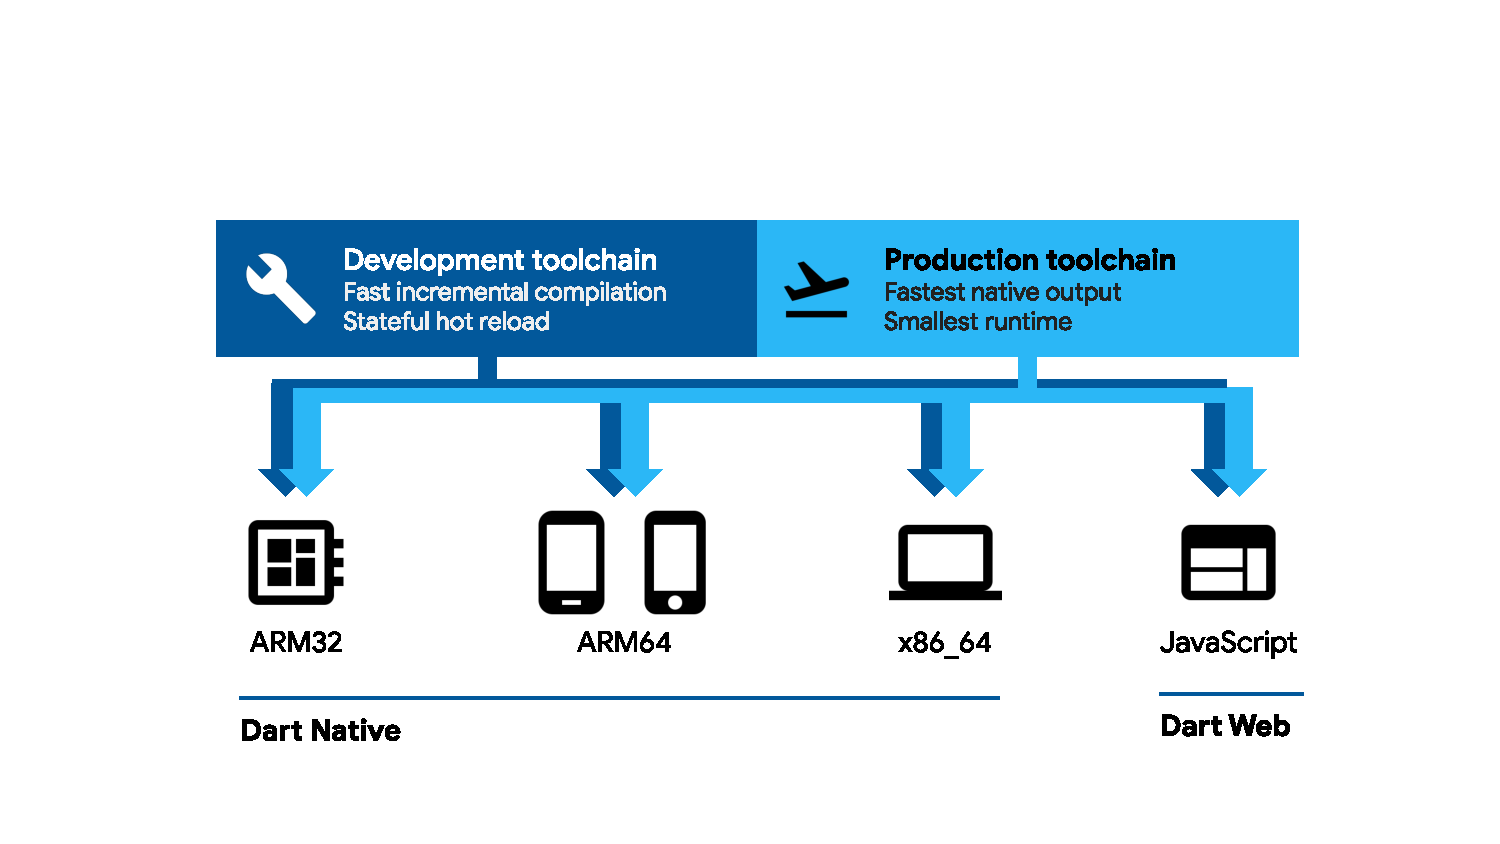
\includegraphics[clip, trim=2.5cm 1cm 0 2cm, width=1.1\textwidth]{dart_build.pdf}
    \caption{Zielplattformen von Dart/Flutter \cite{Dart_Overview}}
    \label{fig:dart_build}
\end{figure}


Dart unterstützt für die native Kompilierung mit \textit{Dart Native} die Verwendung eines \ac{AOT}- oder eines \ac{JIT}-Compilers.
Für \textit{Dart Web} wird der Dart-Code in JavaScript transpiliert und kann somit in Webbrowsern interpretiert werden \cite{Flutter_Architektur}.
Der \ac{JIT}-Compiler ist Teil der \textit{Development toolchain} und wird vor allem während der Entwicklung verwendet um die Build-Zeiten kurz zu halten.
Für die Auslieferung einer in Dart geschriebenen Anwendung wird üblicherweise der \ac{AOT}-Compiler der \textit{Production toolchain} verwendet.
Durch direkte Kompilation in Plattformspezifischen Assembler-Code und zusätzliche Optimierungen werden so im Allgemeinen performantere Anwendungen erzeugt.
Der Wegfall der \ac{JIT}-Kompilierung beim Anwendungsstart sorgt außerdem für schnelle Startzeiten \cite{Dart_Overview}.



Flutter verwendet für die nativen Plattformen eine dreischichtige Architektur.
Wie in \autoref{fig:flutter_architecture} gezeigt, besteht diese aus den Schichten \textit{Framework}, \textit{Engine} und \textit{Embedder}.
Die eigentliche Anwendung wird über der Framework-Schicht umgesetzt und kann die Abstraktionen der darunterliegenden Schicht verwenden.
\begin{figure}[h]
    \centering
    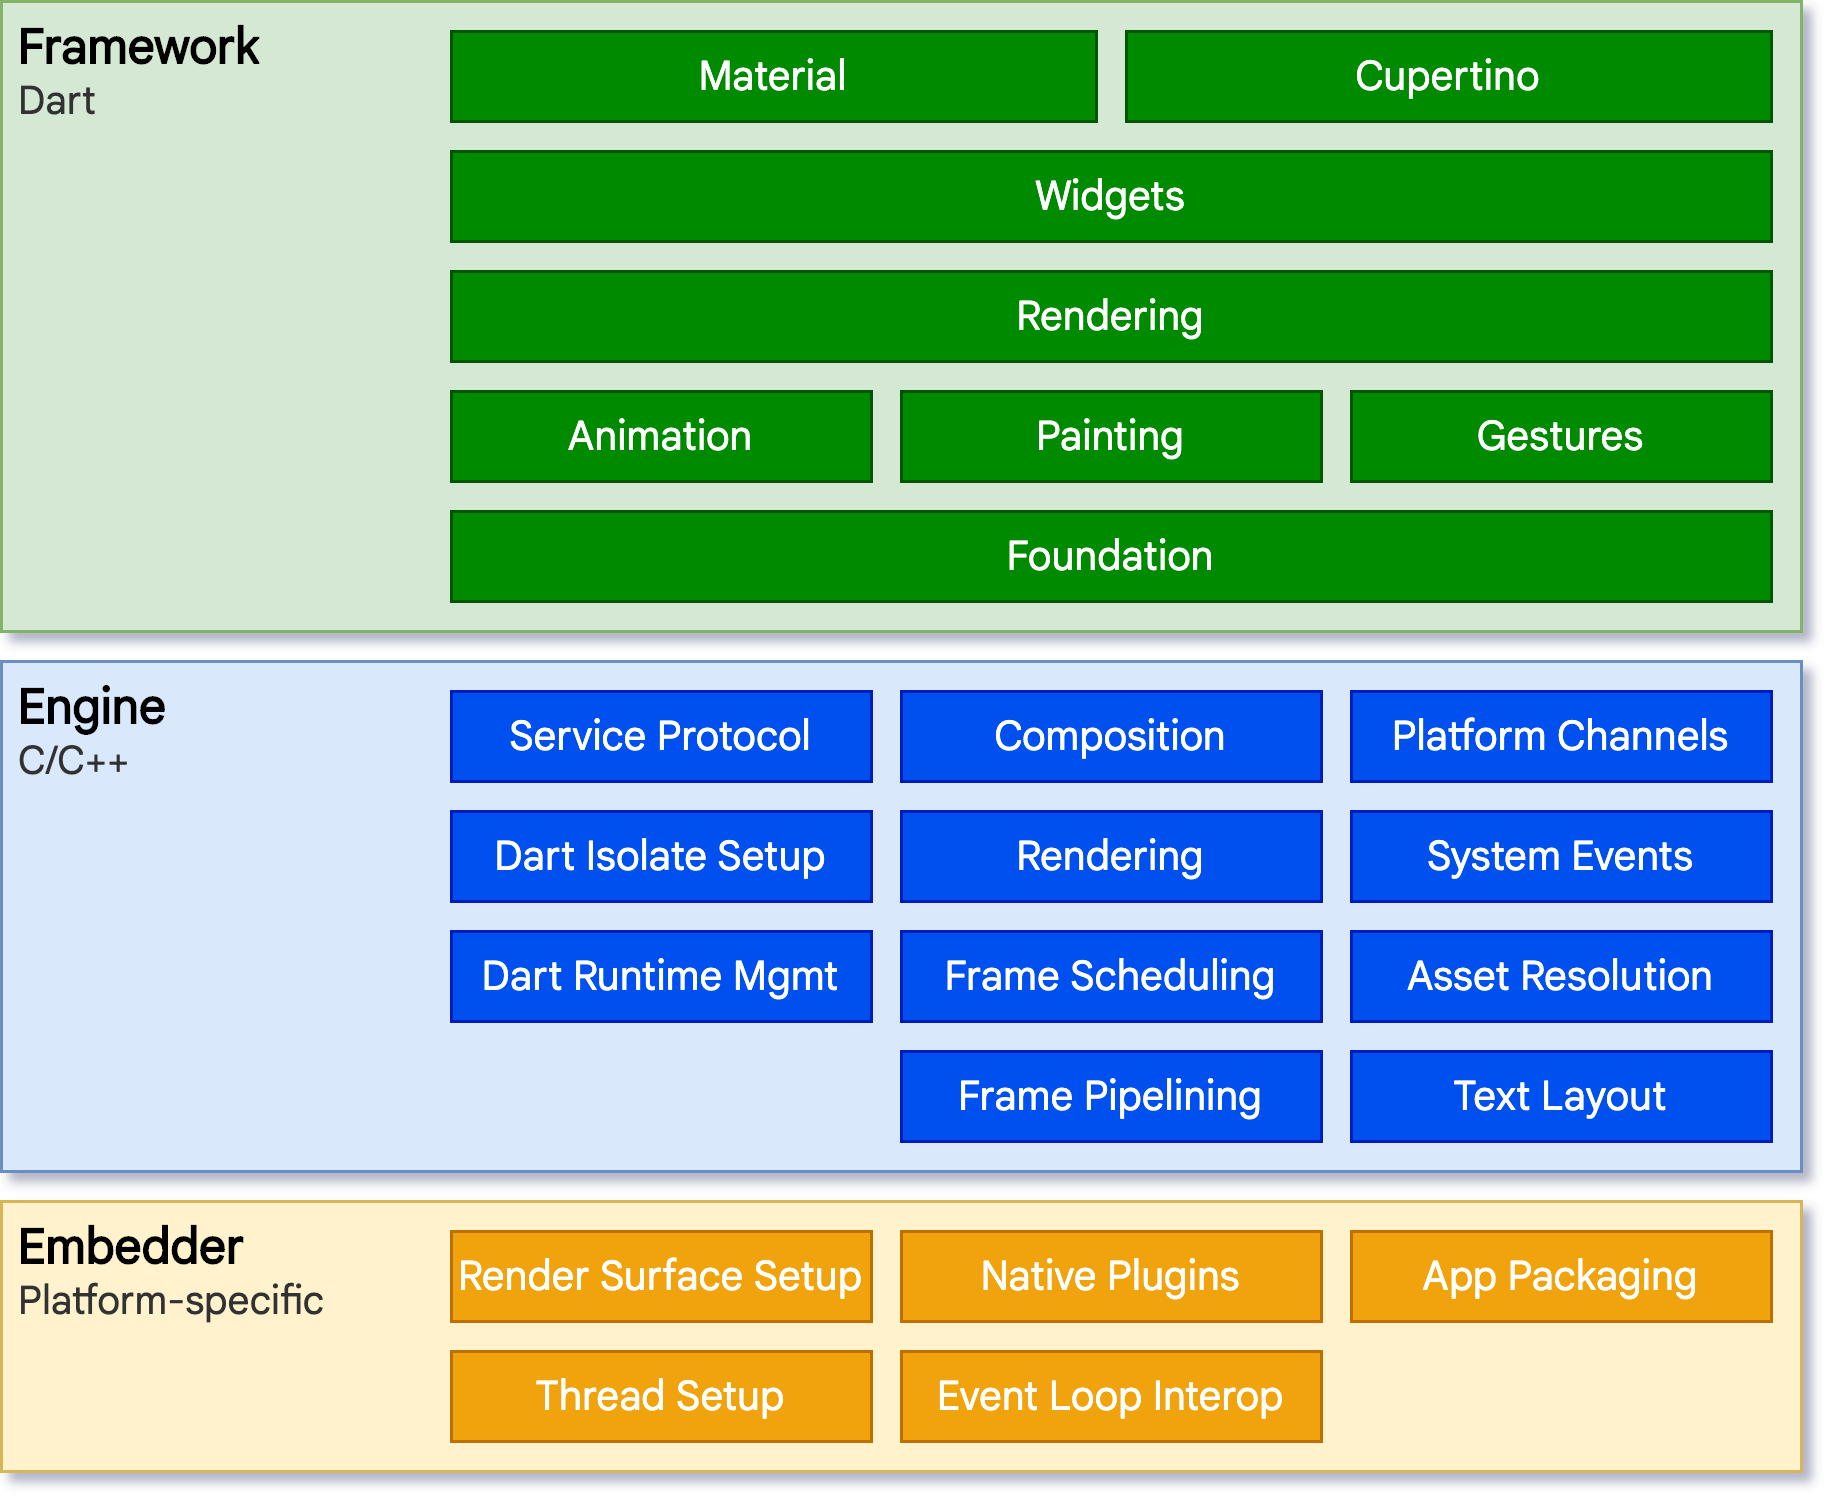
\includegraphics[width=0.9\textwidth]{flutter_architecture.png}
    \caption{Schichtenarchitektur des Flutter-Frameworks \cite{Flutter_Architektur}}
    \label{fig:flutter_architecture}
\end{figure}

Die Basis bildet die Embedder-Schicht, welche als einzige plattformspezifisch ist und der darüber liegenden Schicht eine einheitliche Schnittstelle zum unterlagerten System zur Verfügung stellt.
Für die verbreiteten Plattformen, wie Android und iOS, steht eine Standard-Implementierung bereit.
Zusätzlich können jedoch auch eigene Embedder implementiert werden, um weitere Plattformen zu unterstützen \cite{Flutter_Architektur}.

Auf den Embedder setzt die Flutter-Engine auf, welche die Flutter-\acp{API} bereitstellt und das Rendering der Oberfläche übernimmt.
Anstatt auf die \ac{UI}-Bibliotheken des unterlagerten Systems zurückzugreifen, verwendet Flutter die Skia Graphics Engine um Steuerelemente zu rendern \cite{Biorn-Hansen_PerformanceOverhead_CrossPlatform}.
Skia ist ebenfalls ein Open-Source Projekt und auf allen gängigen Plattformen verfügbar.
Die Engine wird mit jeder Flutter-Anwendung ausgelagert und kann damit mit jedem App-Update aktualisiert werden.
Abhängigkeiten zu einer installierten Version der Skia Engine, welche unter Android standardmäßig verfügbar ist, können so vermieden werden.
Das Flutter-Team gibt an, dass durch den Verzicht auf die Verwendung systemeigener Bibliotheken eine Abstraktionsebene eingespart werden kann, was zu hoher Performance beim \ac{UI}-Rendering führt \cite{Flutter_Architektur}.
Die Framework-Schicht abstrahiert den Zugriff auf die Flutter-Engine und stellt Schnittstellen in Dart bereit.
Außerdem werden auf dieser Ebene verschiedene Bibliotheken bereitgestellt.
Zum Erhalt der Konsistenz des \ac{UI} stehen zum Beispiel die beiden Bibliotheken Material und Cupertino zur Verfügung, welche Steuerelementen im Stil von Google respektive Apple zur Verfügung stellen \cite{Manchanda_CrossPlatformFrameworks, Flutter_Architektur}.


Die Dart-Runtime, in welcher Flutter-Anwendungen ausgeführt werden, erlaubt den Zugriff auf verschiedene wiederverwendbare Bibliotheken, die zum Beispiel \ac{I/O} Funktionen erleichtern \cite{Dart_Overview}.
Darüber hinaus bietet Flutter auch die Möglichkeit, Plattformspezifischen Code aufzurufen, wenn die verfügbaren Bibliotheken nicht ausreichen.
Außerdem existiert eine große Sammlung von Open-Source Plugins, welche den Zugriff auf native Funktionen abstrahieren \cite{Flutter_Architektur,Fentaw_Thesis_Flutter}.


Zur Bewertung der Performance von Flutter existieren widersprüchliche Aussagen.
So gibt es Situationen, in denen Flutter die Performance einer nativen Anwendung sogar übertrifft und ansonsten meist besser abschneidet als Implementierungen mit anderen Frameworks \cite{Nawrocki_Comparison_Hybrid_Native_Frameworks}.
Allerdings zeigen Bi{\o}rn-Hansen \textit{et al.} \cite{Biorn-Hansen_PerformanceOverhead_CrossPlatform}, dass die mittlere Zeit zur Ausführung einer definierten Aufgabe bei mit Flutter entwickelten Apps höher ist als bei äquivalenten Apps, die mit anderen Technologien entwickelt wurden.

Es ist davon auszugehen, dass diese Widersprüche auf verschiedene Anwendungsfälle und unterschiedliche Testmethodiken zurückzuführen sind.
Dementsprechend ist die Performance von Flutter vom konkreten Einsatzzweck und der Zielplattform abhängig.
Weiterhin liefern die genannten Untersuchungen keine Aussagen zur Performance im Anwendungsfall einer Videoaufzeichnung.